\section{Results and discussion}
\label{sec:results}

\subsection{Frequent actor groups}

At $s = 2$ there are 641 frequent actors, 121 frequent pairs, 25 frequent triples and 4 frequent groups of four. Table~\ref{tab:groups} lists the groups of at least two actors with the highest support. They fall into two kinds. Most are the recurring casts of film series: Daniel Radcliffe, Emma Watson and Rupert Grint in the \emph{Harry Potter} films, Carrie Fisher, Harrison Ford and Mark Hamill in \emph{Star Wars}, and Tom Hanks and Tim Allen, who voice the leads of the four \emph{Toy Story} films. The others are long-running collaborations, such as Robert De Niro and Joe Pesci in four films directed by Martin Scorsese (\emph{Raging Bull}, \emph{Goodfellas}, \emph{Casino} and \emph{The Irishman}), and Robert De Niro and Al Pacino. Since 2{,}068 of the 2{,}709 actors appear in a single movie, frequent groups are few and small: no pair appears in more than six movies.

\begin{table}[ht]
  \centering
  \caption{Most frequent groups of at least two actors ($s = 2$).}
  \label{tab:groups}
  \begin{tabular}{lr}
    \toprule
    Actors & Movies \\
    \midrule
    Daniel Radcliffe, Rupert Grint & 6 \\
    Daniel Radcliffe, Emma Watson & 5 \\
    Emma Watson, Rupert Grint & 5 \\
    Daniel Radcliffe, Emma Watson, Rupert Grint & 5 \\
    Joe Pesci, Robert De Niro & 4 \\
    Tim Allen, Tom Hanks & 4 \\
    Al Pacino, Diane Keaton & 3 \\
    Al Pacino, Robert De Niro & 3 \\
    Carrie Fisher, Harrison Ford, Mark Hamill & 3 \\
    \bottomrule
  \end{tabular}
\end{table}

\subsection{Comparison on the original data}

Figure~\ref{fig:original} and Tables~\ref{tab:times} and~\ref{tab:pairs} compare the methods on the original 1000 baskets. Exhaustive counting takes about the same time at every $s$, because it always counts every subset. Basic A-Priori follows its candidate pairs: as $s$ grows from 1 to 10, $|C_2|$ falls from 3{,}667{,}986 to 36 and its time from seconds to about a millisecond, so that it is three orders of magnitude slower than exhaustive counting at $s = 1$ and faster from $s = 5$. Optimized A-Priori stores only the pairs that occur and is the fastest method from $s = 2$ upwards, level with basic A-Priori at $s = 10$, where little remains to prune. At $s = 1$ every subset of every basket is frequent and nothing can be pruned, so A-Priori only pays for its extra passes and exhaustive counting is faster.

\begin{figure}[ht]
  \centering
  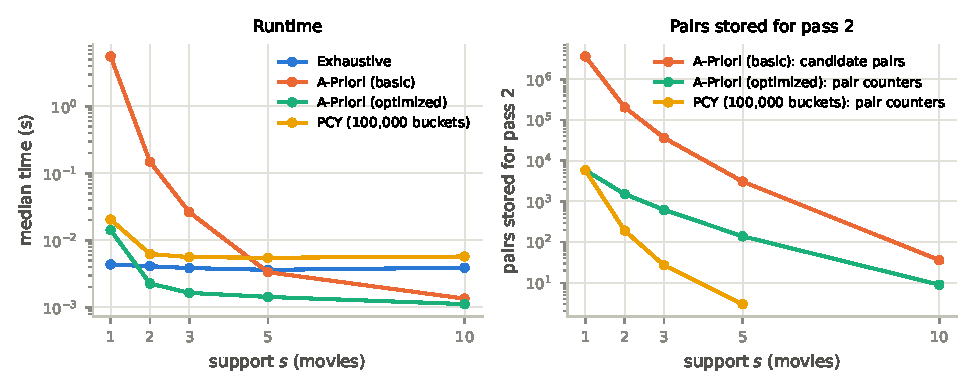
\includegraphics[width=\textwidth]{figures/original.pdf}
  \caption{Original data. Left: median time per method (log scale). Right: pairs stored for pass 2, the candidate pairs for basic A-Priori and the pair counters for the other methods (log scale; PCY stores no pairs at $s = 10$).}
  \label{fig:original}
\end{figure}

\begin{table}[ht]
  \centering
  \caption{Median time (ms) on the original data (reference run).}
  \label{tab:times}
  \begin{tabular}{rrrrrrrr}
    \toprule
    & & \multicolumn{2}{c}{A-Priori} & \multicolumn{4}{c}{PCY, $B =$} \\
    \cmidrule(lr){3-4} \cmidrule(lr){5-8}
    $s$ & exhaustive & basic & optimized & $10^3$ & $10^4$ & $10^5$ & $10^6$ \\
    \midrule
    1 & 4.4 & 5{,}581 & 14.2 & 16.8 & 16.9 & 20.5 & 50.0 \\
    2 & 4.1 & 149 & 2.3 & 3.7 & 3.8 & 6.3 & 33.6 \\
    3 & 3.9 & 26.3 & 1.6 & 2.9 & 3.0 & 5.6 & 32.5 \\
    5 & 3.6 & 3.4 & 1.4 & 2.5 & 2.7 & 5.5 & 32.5 \\
    10 & 3.9 & 1.3 & 1.1 & 2.5 & 2.5 & 5.7 & 32.9 \\
    \bottomrule
  \end{tabular}
\end{table}

\begin{table}[ht]
  \centering
  \caption{Pairs stored for pass 2 on the original data: candidate pairs for basic A-Priori, pair counters for the other methods.}
  \label{tab:pairs}
  \begin{tabular}{rrrrrrr}
    \toprule
    & \multicolumn{2}{c}{A-Priori} & \multicolumn{4}{c}{PCY, $B =$} \\
    \cmidrule(lr){2-3} \cmidrule(lr){4-7}
    $s$ & basic & optimized & $10^3$ & $10^4$ & $10^5$ & $10^6$ \\
    \midrule
    1 & 3{,}667{,}986 & 5{,}833 & 5{,}833 & 5{,}833 & 5{,}833 & 5{,}833 \\
    2 & 205{,}120 & 1{,}516 & 1{,}508 & 696 & 192 & 129 \\
    3 & 36{,}585 & 622 & 612 & 82 & 27 & 25 \\
    5 & 3{,}081 & 139 & 120 & 5 & 3 & 3 \\
    10 & 36 & 9 & 1 & 0 & 0 & 0 \\
    \bottomrule
  \end{tabular}
\end{table}

PCY needs the fewest pair counters, and the more buckets it has, the closer it gets to the frequent pairs: at $s = 2$ it counts 1{,}508 pairs with $10^3$ buckets, where the average bucket count $P / B \approx 6$ exceeds $s$ and almost every bucket is frequent, and 129 with $10^6$, against 121 frequent pairs. At $s = 1$ every occurring pair is frequent and nothing can be filtered. It is nevertheless slower than optimized A-Priori in every configuration: pass 1 hashes every pair of every basket, and creating and scanning the buckets adds a cost that grows with $B$ and dominates with $10^6$ buckets. As noted in Section~\ref{sec:algorithms}, its advantage is a smaller set of pair counters, not time, and in this implementation not total memory either.

\subsection{Scalability}

Figure~\ref{fig:scaling} shows the median time as the data grows at $s = 2$, and Table~\ref{tab:exponents} the fitted growth exponents.

\begin{figure}[ht]
  \centering
  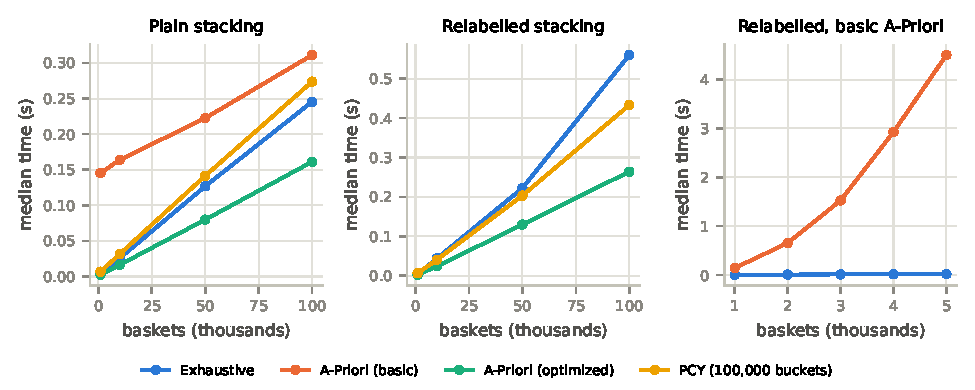
\includegraphics[width=\textwidth]{figures/scaling.pdf}
  \caption{Median time against the number of baskets at $s = 2$. Left: plain stacking. Centre: relabelled stacking. Right: basic A-Priori on relabelled stacking, run only up to five copies.}
  \label{fig:scaling}
\end{figure}

\begin{table}[ht]
  \centering
  \caption{Growth exponents $\alpha$ of the median time, $t \propto n^{\alpha}$ (reference run).}
  \label{tab:exponents}
  \begin{tabular}{lrrrr}
    \toprule
    & \multicolumn{2}{c}{plain stacking} & \multicolumn{2}{c}{relabelled stacking} \\
    \cmidrule(lr){2-3} \cmidrule(lr){4-5}
    Method & $s = 2$ & $s = 5$ & $s = 2$ & $s = 5$ \\
    \midrule
    Exhaustive & 0.98 & 0.97 & 1.09 & 1.06 \\
    A-Priori (basic) & 0.26 & 0.94 & 2.12 & -- \\
    A-Priori (optimized) & 0.99 & 1.00 & 1.05 & 1.00 \\
    PCY ($B = 10^3$) & 1.00 & 1.01 & 1.08 & 1.05 \\
    PCY ($B = 10^4$) & 0.98 & 0.97 & 1.06 & 1.05 \\
    PCY ($B = 10^5$) & 0.94 & 0.93 & 1.02 & 1.06 \\
    PCY ($B = 10^6$) & 0.72 & 0.67 & 0.85 & 0.76 \\
    \bottomrule
  \end{tabular}
\end{table}

Under plain stacking the frequent itemsets do not change, and exhaustive counting, optimized A-Priori and PCY grow approximately linearly ($\alpha \approx 1$), as the pass structure predicts. Two cases grow more slowly because a fixed cost is still a large share of their time at these sizes: basic A-Priori at $s = 2$, whose 205{,}120 candidate pairs cost the same at every size ($\alpha = 0.26$), and PCY with $10^6$ buckets, whose buckets do ($\alpha \approx 0.7$). Optimized A-Priori is the fastest method at every size.

Under relabelled stacking the frequent actors grow with the data. Optimized A-Priori and PCY still grow approximately linearly, because they only create counters for pairs that occur, whose number grows linearly as well. Exhaustive counting also grows linearly but is about twice as slow as under plain stacking, because its table of distinct subsets grows $r$-fold. Basic A-Priori grows with $\alpha = 2.12$, slightly faster than quadratically, consistent with $|C_2| \approx r^2 \binom{m}{2}$: this is what RU calls the ``tyranny of counting pairs'' (\S6.2.4).

\begin{table}[ht]
  \centering
  \caption{Pair counters for pass 2 under relabelled stacking.}
  \label{tab:pcy-relabelled}
  \begin{tabular}{rrrrrr}
    \toprule
    & & & \multicolumn{3}{c}{PCY, $B =$} \\
    \cmidrule(lr){4-6}
    $s$ & baskets & A-Priori (optimized) & $10^4$ & $10^5$ & $10^6$ \\
    \midrule
    2 & 1{,}000 & 1{,}516 & 696 & 192 & 129 \\
    2 & 10{,}000 & 15{,}160 & 15{,}122 & 7{,}325 & 1{,}941 \\
    2 & 50{,}000 & 75{,}800 & 75{,}800 & 72{,}549 & 22{,}263 \\
    2 & 100{,}000 & 151{,}600 & 151{,}600 & 151{,}432 & 72{,}676 \\
    \midrule
    5 & 1{,}000 & 139 & 5 & 3 & 3 \\
    5 & 10{,}000 & 1{,}390 & 1{,}184 & 50 & 30 \\
    5 & 50{,}000 & 6{,}950 & 6{,}950 & 2{,}789 & 150 \\
    5 & 100{,}000 & 13{,}900 & 13{,}900 & 11{,}932 & 413 \\
    \bottomrule
  \end{tabular}
\end{table}

Relabelled stacking also exposes the limit of PCY (Table~\ref{tab:pcy-relabelled}). The pair occurrences grow to $r\,P$, so for a fixed $B$ the average bucket count $r P / B$ grows with the data. With $10^5$ buckets PCY removes most pairs on the original data, but at 100{,}000 baskets the average bucket count is about 6, above $s = 2$, and PCY still counts 151{,}432 of the 151{,}600 pairs of optimized A-Priori. With $10^6$ buckets the average is about 0.6, and PCY still removes about half of the pairs at $s = 2$ and 97\% at $s = 5$. As RU Example~6.9 suggests, the number of buckets must grow with the pair occurrences for the filter to remain effective.
